% ---------------------------------------------------------
\subsection{Architecture}
% ---------------------------------------------------------

The benchmark program follows a layered architecture pattern. Each layer represents a
distinct subsystem that is responsible for a specific set of tasks and clearly defined
responsibilities.
This architectural approach enables flexible combinations of workloads and optimizers.
Furthermore, the system can be extended beyond machine learning workloads to support
other computational tasks for performance evaluation.  
Figure \ref{fig:architecture-overview} illustrates an overview of the architecture and
its modules.

\begin{figure}[h]
	\centering
	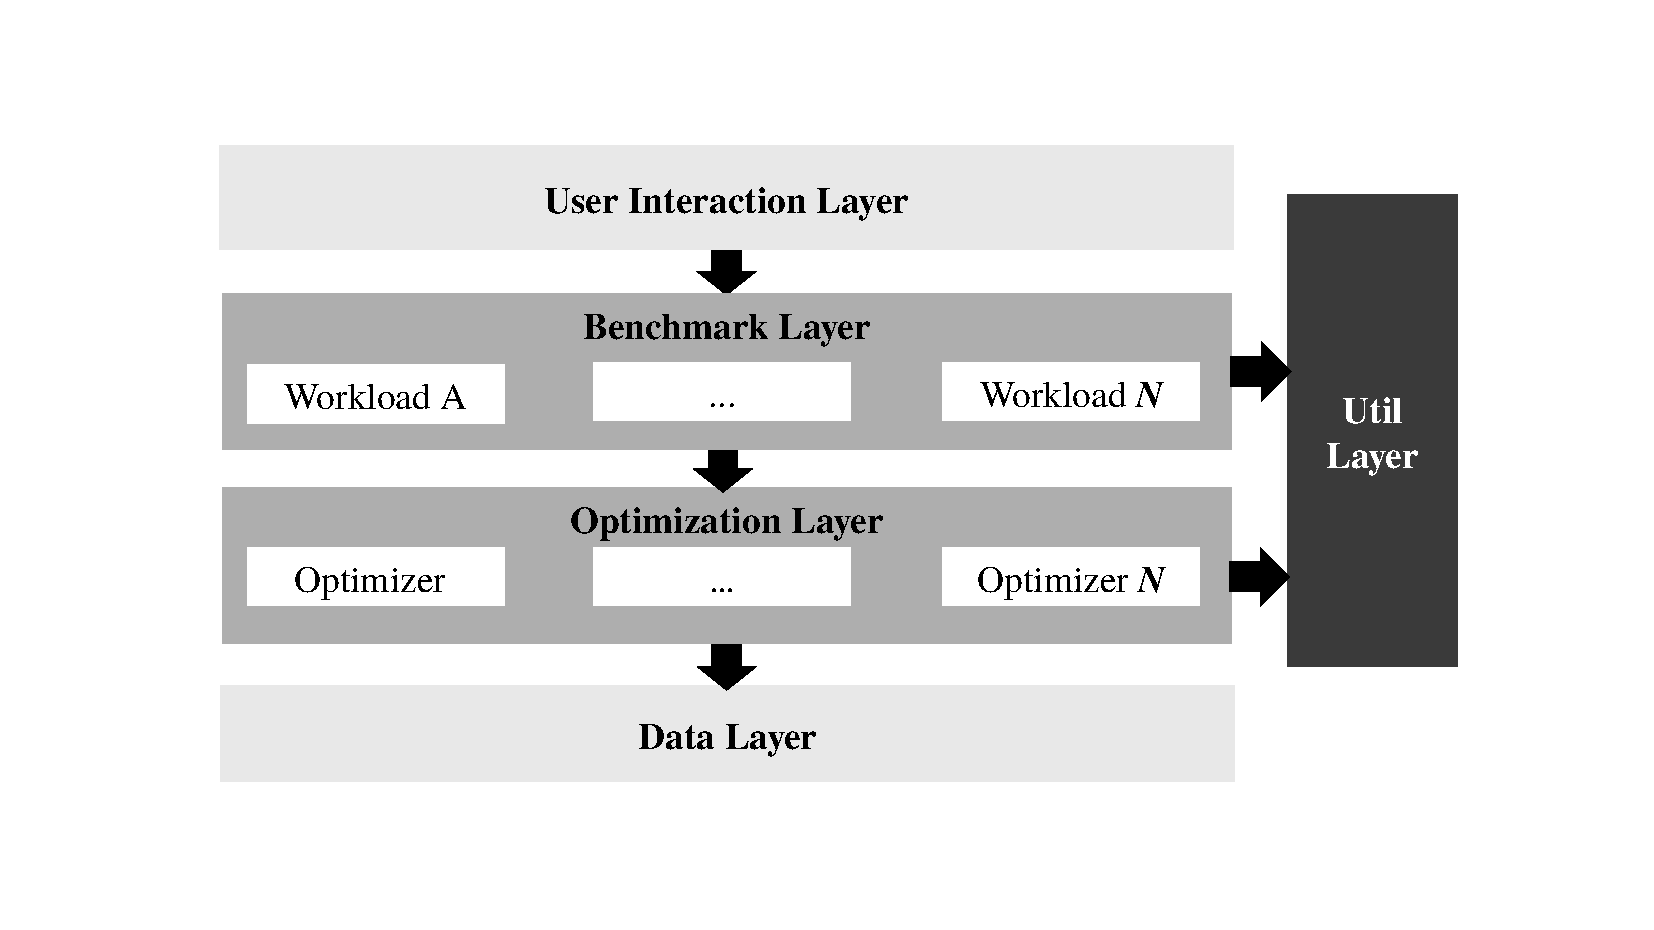
\includegraphics[width=17cm,height=10cm]{diagrams/umls/architecture-overview.pdf}
	\caption{Layered architecture of the benchmark system. The User Interaction Layer
	(implemented as a CLI) communicates with the Benchmark Layer, which manages
	multiple workloads. The Optimization Layer provides different optimizers that
	execute these workloads. All layers rely on shared functionality provided by
	the Util Layer.}
	\label{fig:architecture-overview}
\end{figure}

User interaction is handled through the command-line interface (CLI), which
allows users to configure and execute benchmark experiments. The CLI abstracts low-level
system interactions and provides a simple and consistent interface.
The Benchmark Layer is responsible for defining and managing benchmark executions.
Each workload represents a specific computational task that is executed by an optimizer.
This layer initializes workloads and provides the required configuration to the
Optimization Layer.
The Optimization Layer contains the implementations of the optimizers that execute the
workloads. These optimizers encapsulate the optimization logic and performance-critical
computations.
All layers interact with the Util Layer, which provides shared functionality such as
wrapper classes, logging mechanisms, and other cross-cutting utilities.

The following subsections describe each layer in more detail.

% ---------------------------------------------------------
\subsubsection{Benchmark Layer}
% ---------------------------------------------------------

The Benchmark Layer serves as the entry point of the application and is responsible
for defining and executing different workloads. The layer consists of two main modules:
the benchmark module and the workload module.

\begin{figure}[h]
	\centering
	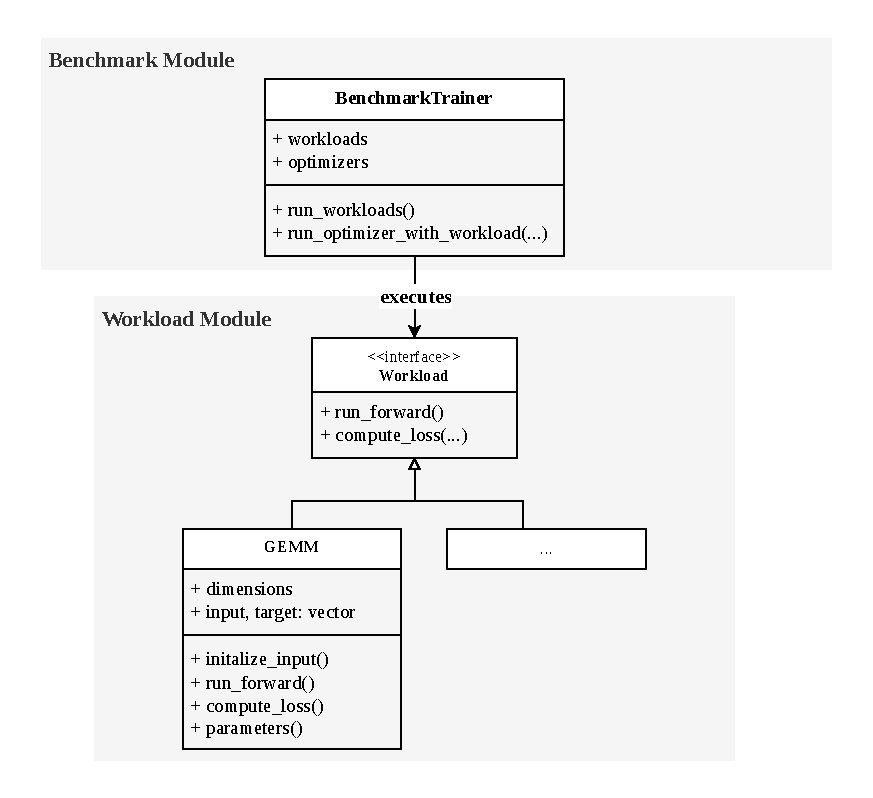
\includegraphics[width=14cm,height=14cm]{diagrams/umls/benchmark-layer-uml.pdf}
	\caption{Domain-agnostic implementation of workloads. The design enables
	maintainable integration of additional workloads in the future.}
	\label{fig:benchmark-layer}
\end{figure}

Figure \ref{fig:benchmark-layer} illustrates the implementation of the Benchmark Layer.
The class \verb|BenchmarkTrainer| is responsible for allocating the workload and
executing all required preprocessing steps before running the optimizer.
Each workload implements the abstract class or interface \verb|Workload|.
This design provides a domain-agnostic abstraction that decouples the workload
implementation from the optimization and benchmarking logic. As a result,
the benchmark program can support a wide variety of workloads.
Within the scope of this project, the class \verb|GEMM| implements a simple
neural-network workload consisting of a forward pass only. Since the current
implementation does not perform learning via backpropagation and instead only
executes forward propagation, the workload is effectively equivalent to a
general matrix multiplication (GEMM) operation rather than a full machine
learning training process.

The primary purpose of this workload is therefore to evaluate the performance
of large matrix multiplications that are transferred to and executed on the GPU
during optimization.

% ---------------------------------------------------------
\subsubsection{Optimization Layer}
% ---------------------------------------------------------

In addition to initializing workloads, the class \verb|BenchmarkTrainer|
also applies a selected optimizer to the workload.

The Optimization Layer follows a design similar to the Benchmark Layer,
allowing multiple optimizer implementations to be integrated and combined
with different workloads.

\begin{figure}[h]
	\centering
	
\includegraphics[width=14cm,height=14cm]{diagrams/umls/optimization-layer-uml.pdf}
	\caption{Domain-agnostic optimizer architecture. Different optimizer
	implementations can be provided for specific execution platforms.}
	\label{fig:optimization-layer}
\end{figure}

Figure \ref{fig:optimization-layer} shows the implementation concept of the
Optimization Layer. Each optimizer implements the abstract class or interface
\verb|Optimizer|.
All optimizer implementations must provide an implementation of the
\verb|step| function. This function is executed during each iteration of the
training or optimization process and updates the parameters toward a local
or global optimum.
For example, the Adam optimizer is implemented in the classes
\verb|AdamOptimizer|, \verb|AdamOptimizerCl| (OpenCL), and
\verb|AdamOptimizerCu| (CUDA). In this case, the \verb|step| function performs
a parameter update in the parameter space at time step $t$, as described by
Kingma and Ba \cite{adam}.
Because data transfer to GPU devices differs between frameworks,
additional functions such as \verb|fromDevice| or
\verb|launch_adam_kernel| are required to manage device-specific execution.

% ---------------------------------------------------------
\subsubsection{Util Layer}
% ---------------------------------------------------------

The Util Layer provides shared functionality that is used throughout the
entire project. These utilities address cross-cutting concerns such as
data representation, logging, and framework abstraction.

\begin{figure}[h]
	\centering
	
\includegraphics[width=14cm,height=14cm]{diagrams/umls/util-layer.pdf}
	\caption{Utility layer components providing shared functionality
	across the application.}
	\label{fig:util-layer}
\end{figure}

Figure \ref{fig:util-layer} illustrates the interactions between the
different utility components. Data view classes such as
\verb|HostParamsView| and \verb|DeviceParamView| provide platform-specific
representations of parameter data.
Since OpenCL and CUDA require different data representations for GPU
execution, parameter data must be converted from the host representation
(\verb|HostParamsView|) to the device representation
(\verb|DeviceParamView|). This conversion is handled by the respective
optimizer implementations.
Furthermore, optimizer classes interact with wrapper classes that
encapsulate OpenCL and CUDA functionality. These wrappers significantly
reduce the amount of boilerplate code required to execute workloads on
GPU devices.
At the end of each benchmark execution, the collected benchmark results,
stored in the \verb|benchmarkData| class, are written to a CSV file.
This process is handled by the \verb|Logger| class.

% ---------------------------------------------------------
\subsubsection{Data Layer}
% ---------------------------------------------------------

The Data Layer consists of the benchmark CSV file that stores the results
of all benchmark executions. These results can later be used for further
analysis.
A snippet of the file is shown in Listing \ref{listing:benchmark-data}.

\begin{verbatim}
timestamp,framework,workload_name,workload_type,device,batch_size,input_size,optimizer,learning_rate,beta1,beta2,epsilon,time_ms,batch_index,loss
2026-02-02-11-13-36,None,GEMM_Adam_CPU,compute,CPU,10,1048723456,Adam,0.001,0.9,0.999,1e-08,113,1,0
2026-02-02-11-13-41,None,GEMM_Adam_CPU,compute,CPU,10,1048723456,Adam,0.001,0.9,0.999,1e-08,83,2,0.0224746
...
\end{verbatim}

The goal of the logging system is to capture as much contextual information
as possible from each benchmark execution. Most of the recorded data
describes the experimental configuration, including hyperparameters such as
\verb|learning_rate|, \verb|beta1|, and \verb|beta2|.
The actual performance measurement is represented by the variable
\verb|time_ms|. However, including the surrounding context allows a more
detailed analysis of potential correlations between execution conditions
and performance characteristics.
